
\end{multicols}

\pagebreak
\begin{multicols}{2}[\section{Architecture}]

\label{sec:architecture}

The following section will briefly overview the architecture of our software.

\end{multicols}
\begin{multicols}{2}[\subsection{Overview}]
\label{sec:architecture-overview}

Early on we divided our software into two major components, which – seen individually – should be able to run as stand alone applications as well as as integrated components. This approach should give us the ability to work on different parts of the software more independently. Furthermore, since both components are largely decoupled, it would be easier changing one of them without breaking the other.

These two components are:
\begin{description}
\item[A scheduler] which provides for an automatic allocation of courses to rooms and times.
\item[A web application] which is splitted into three tiers:
	\begin{itemize}
	\item The front end
	\item A controlling unit \emph{(controller)}
	\item The business logic
	\end{itemize}
\end{description}

Both components should work on common ground, which emerges naturally from the need for both to work on the same data. Thus they were to access the same database and we decided to create a data access layer which should be shared by both components.

\begin{figure}[H]
	\centering
		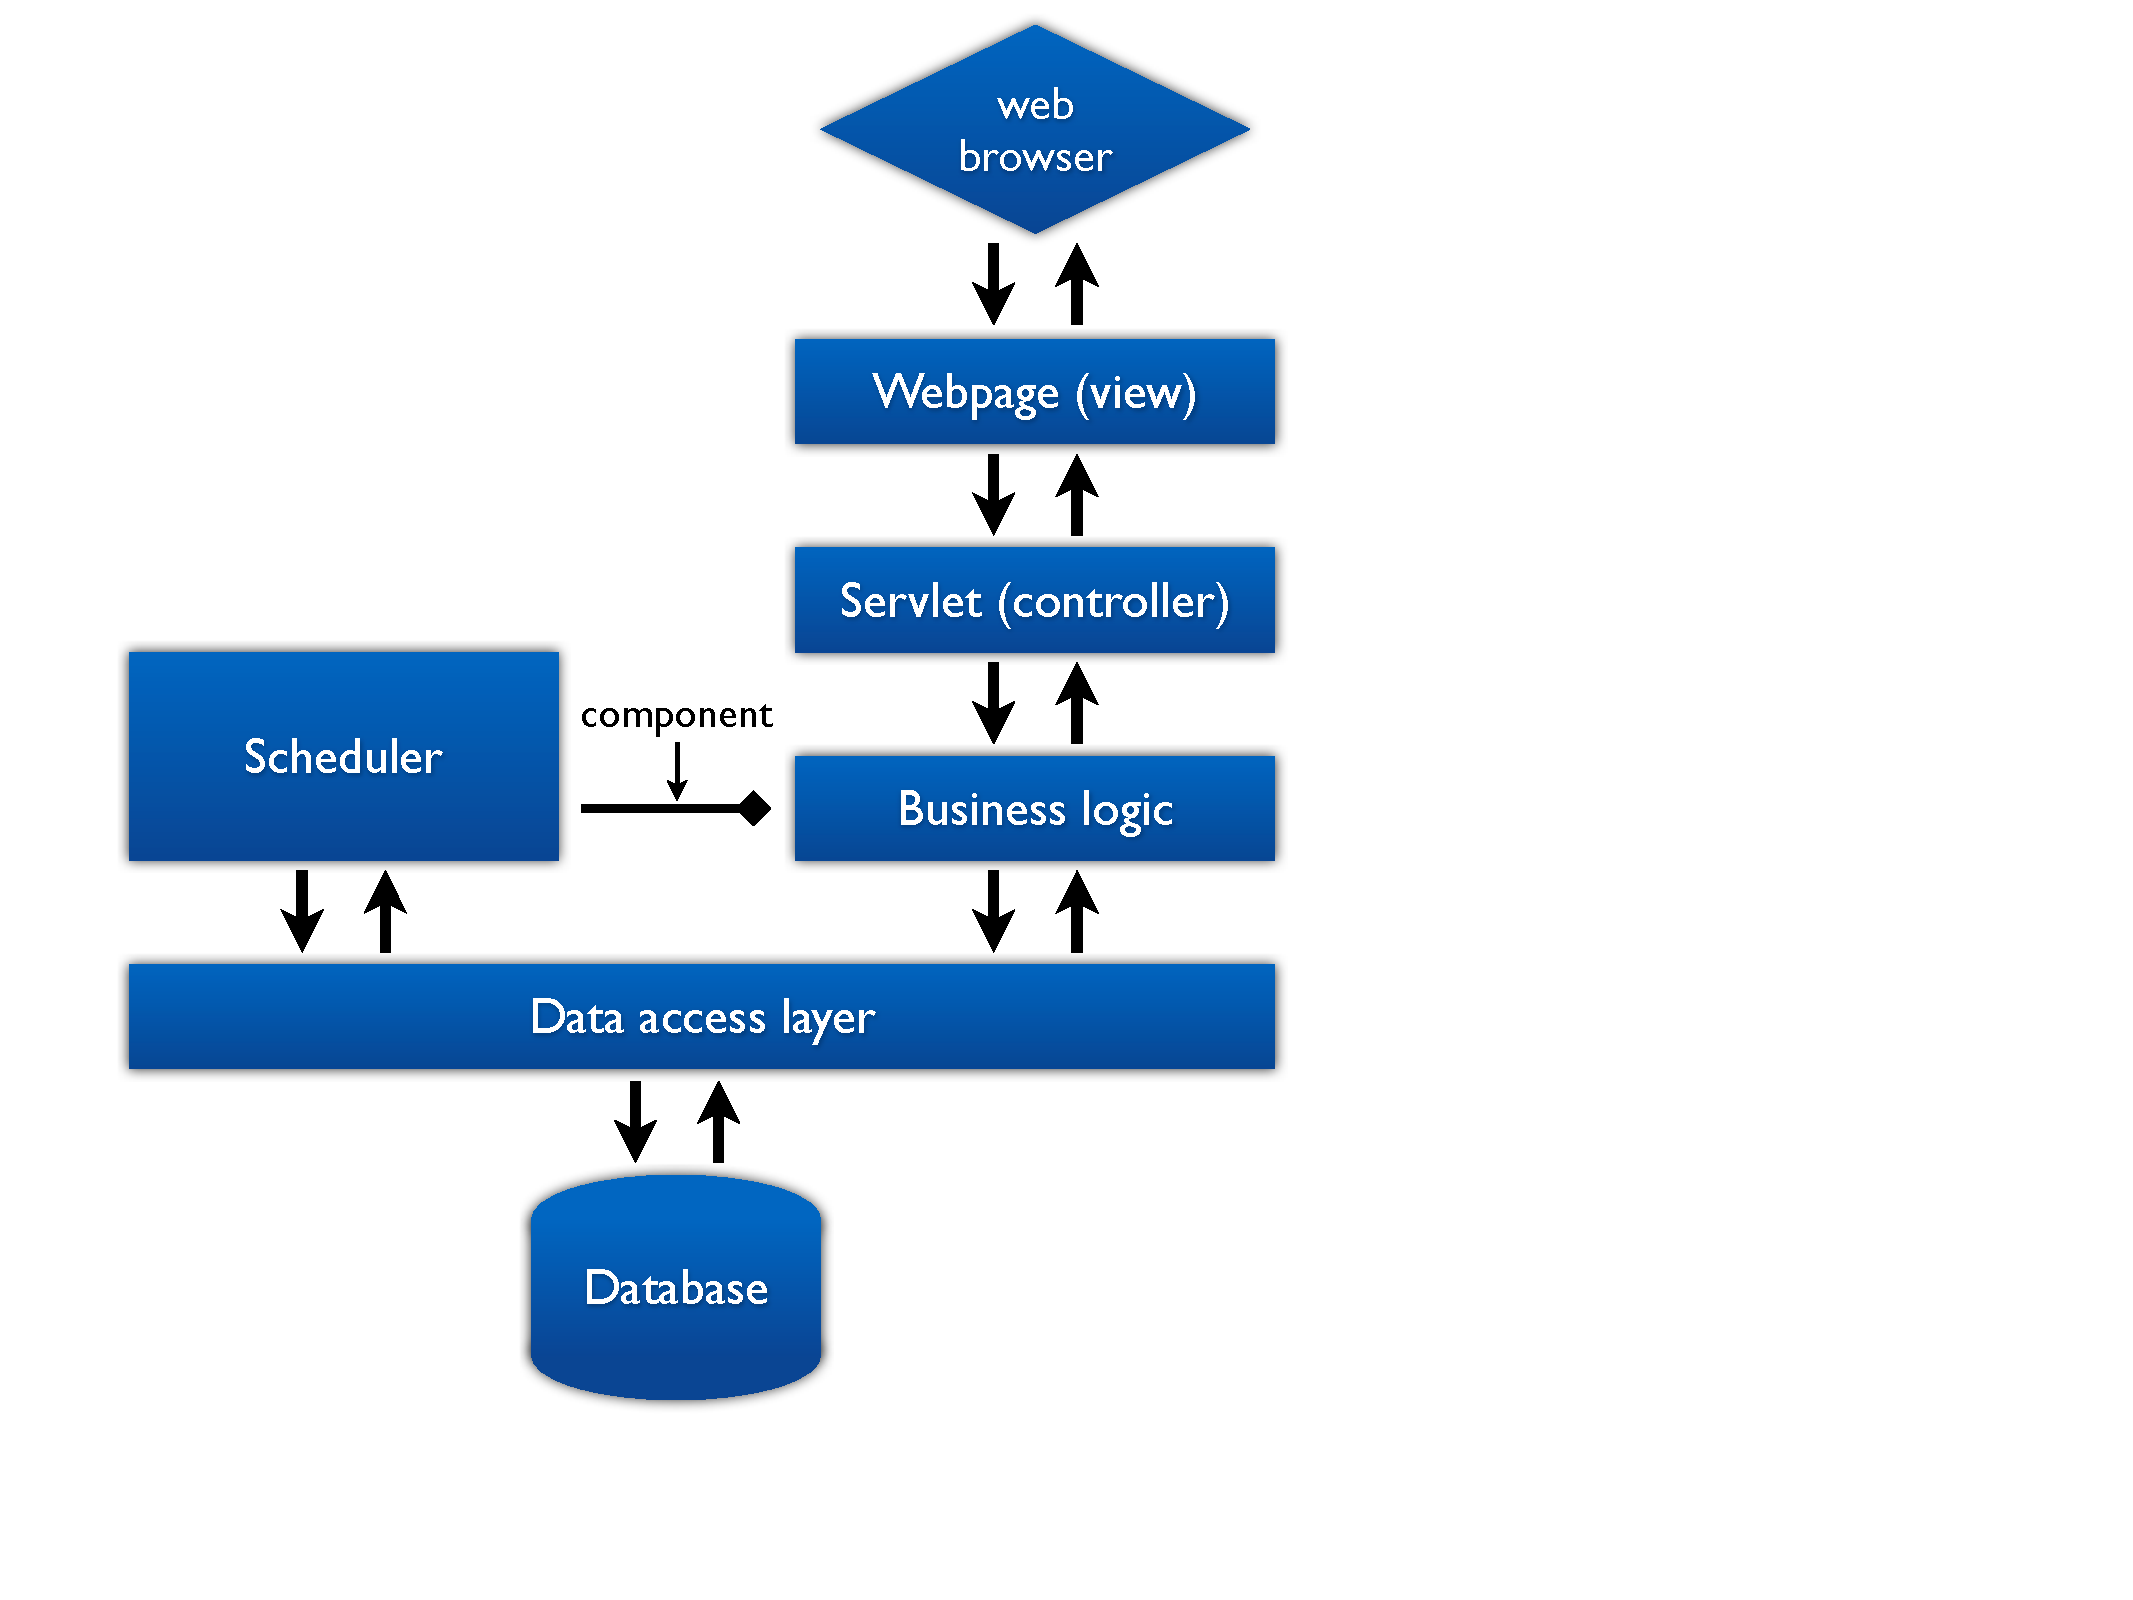
\includegraphics[width=\columnwidth]{images/architecture.pdf}
		\caption{An overview of the components}
	\label{fig:architecture}
\end{figure}


\end{multicols}
\begin{multicols}{2}[\subsection{Data access layer}]
\label{sec:architecture-data-access-layer}

In order to create a proper model of the entities we were to work with, we decided to develop an object-relational model. By that we understand a model which can easily be mapped to an object-oriented model, as well as an entity-relationship-model\footnote{Not to be confused with approaches to store objects in relational databases} from which the object-oriented classes as well as an entity-relationship database definition can be derived.

\begin{figure}[H]
	\centering
		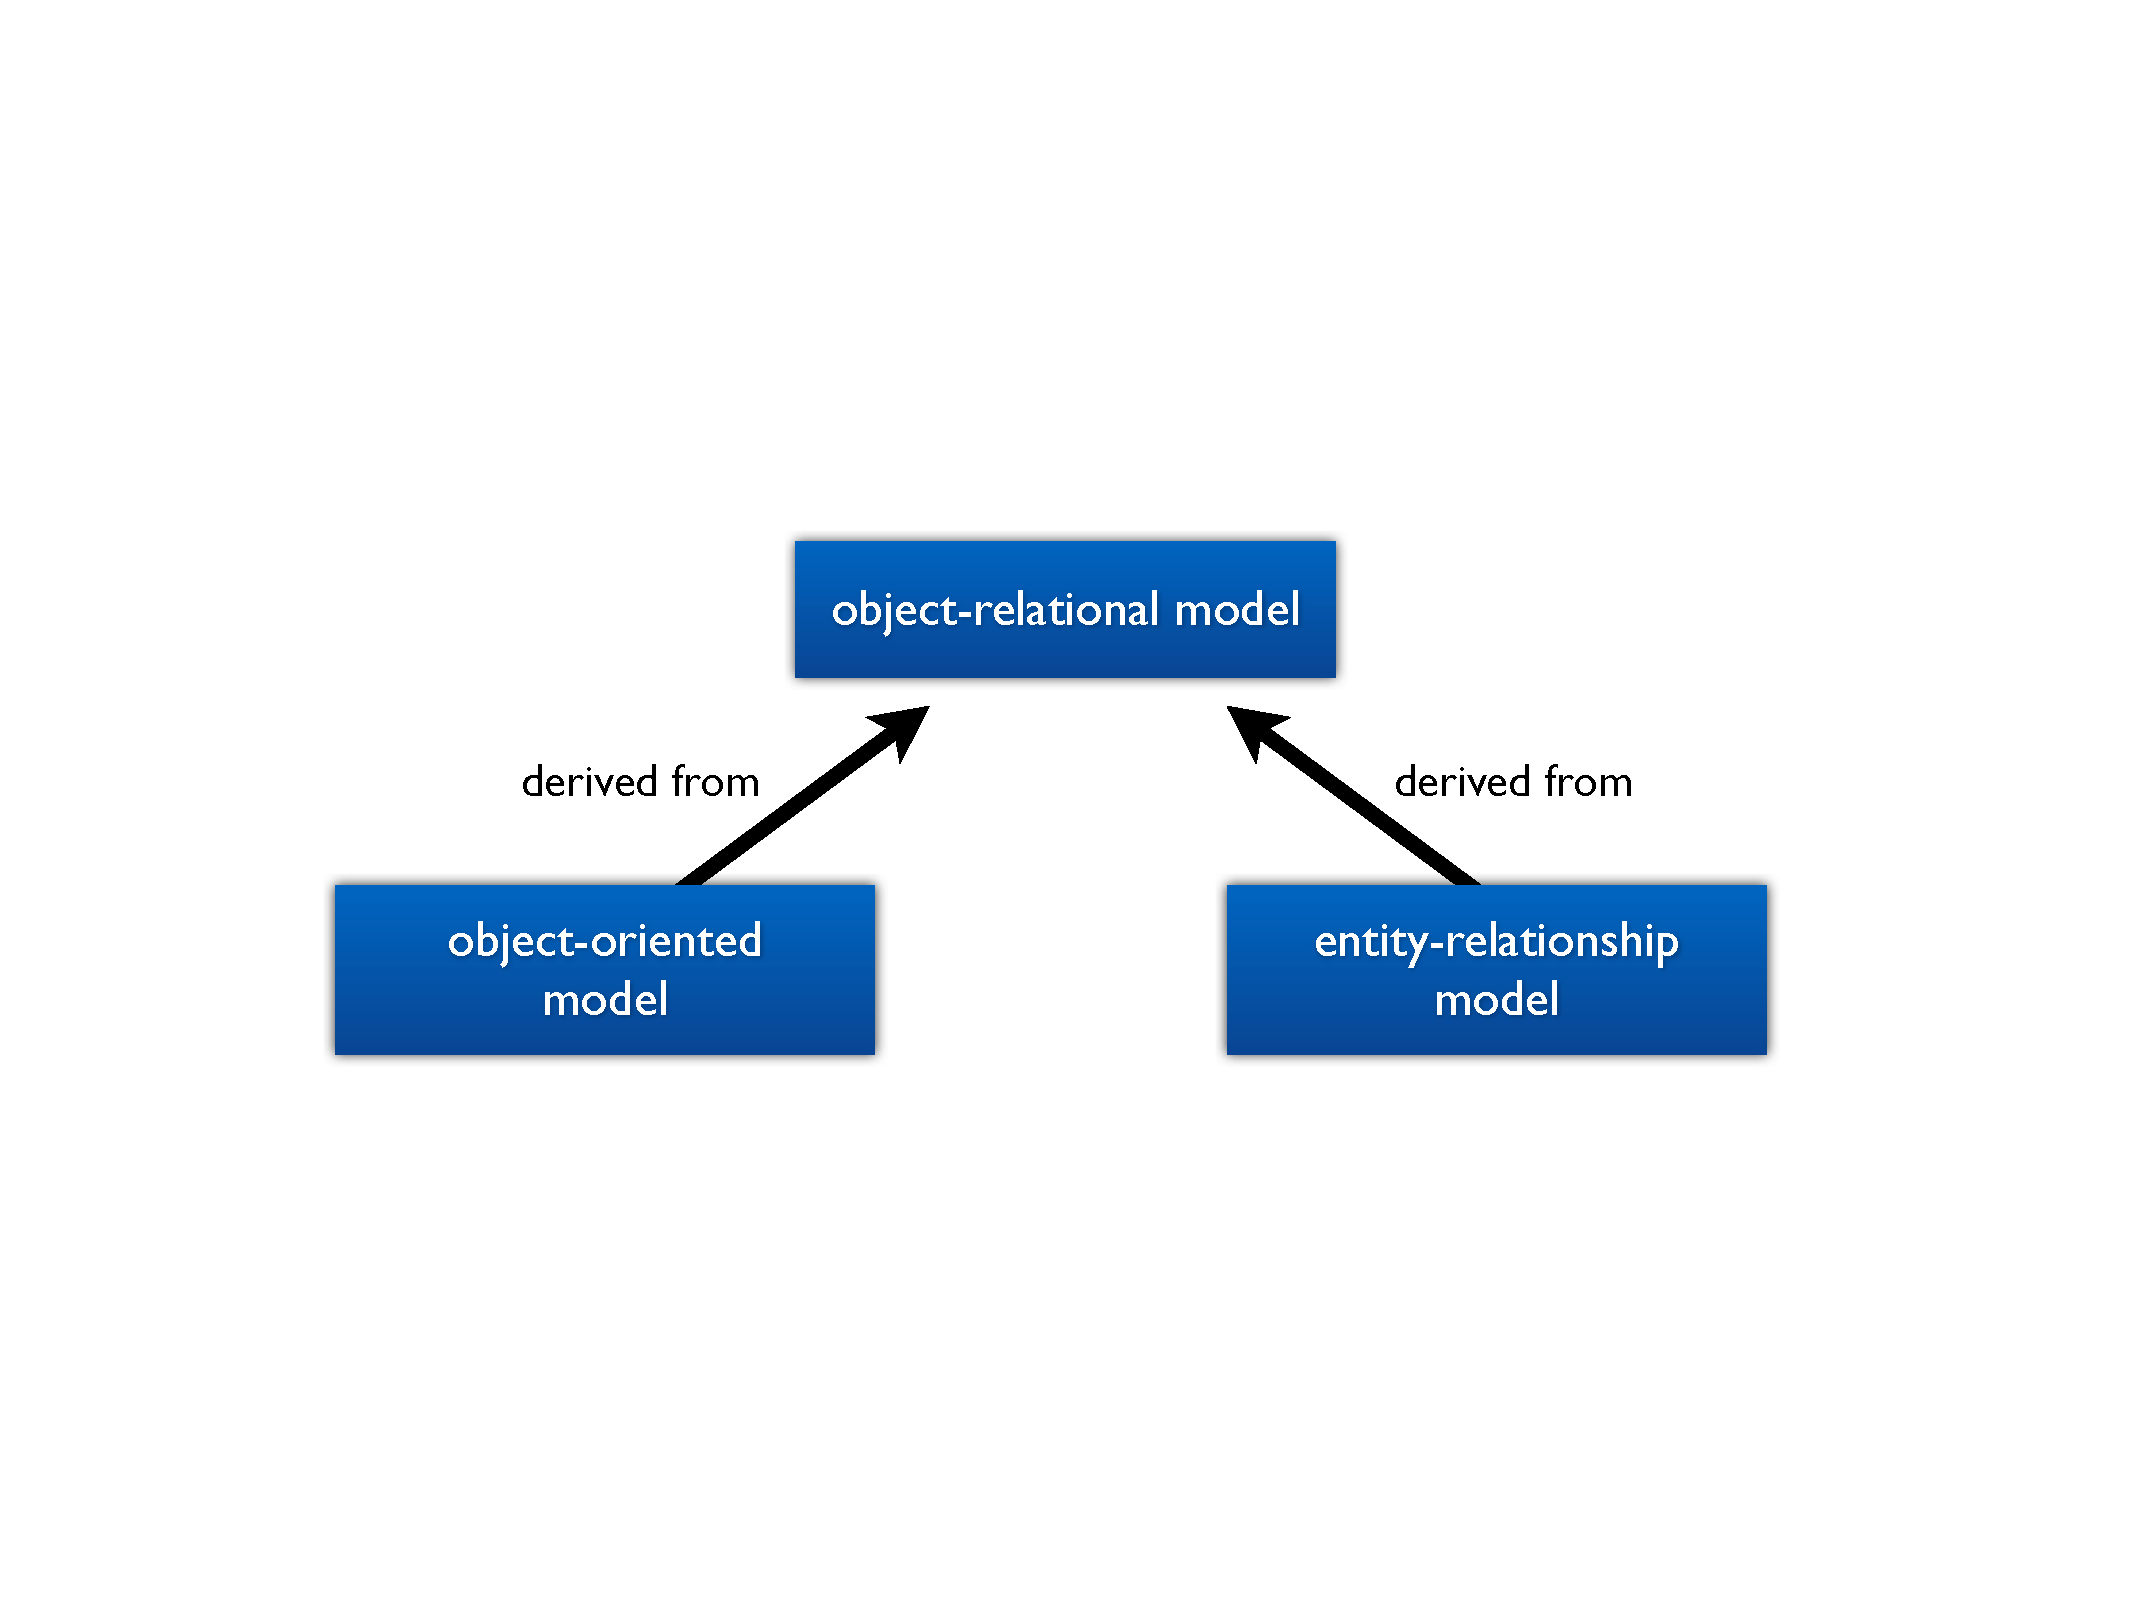
\includegraphics[width=\columnwidth]{images/model.pdf}
		\caption{The object-oriented model and the entity-relationship oriented model are derived from the object-relational model. Since both the OO as well as the ER model derive from the same basic model, they are guaranteed to be in a consistent state.}
	\label{fig:model}
\end{figure}


\end{multicols}
\begin{multicols}{2}[\subsection{Scheduler}]

For providing a reasonably fast pre-scheduling, we wanted to use a genetic algorithm. Such algorithms roughly consist of three parts:

\begin{description}
\item[A fitness function] which evaluates the quality of an intermediate solution.

\item[A cross over function] which intermixes two intermediate solutions in a specific manner in order to create a better solution.

\item[A mutation function] which randomly or intelligently refactors an intermediate solution.

\item[The algorithm itself] which controls the execution of the other parts, i.e. in what order the components are applied and how many intermediate solutions are created.

\end{description}

We decided to model these parts as exchangable components, i.e. individual objects, which could be combined in any way. Since we did not have any experience with these kind of algorithms this design should help us to better understand and scale the different parts of the algorithm.

\label{sec:architecture-scheduler}


